% !TEX TS-program = pdflatex
% !TEX encoding = UTF-8 Unicode

% This is a simple template for a LaTeX document using the "article" class.
% See "book", "report", "letter" for other types of document.

%%%%%%%%%%%%%%%%%%%%%%%%%%%%%%%%%%%%%
%
% Template para producir documentos "camera ready" para Anales de la AFA
% 
%  No se debería tener que modificar nada del siguiente preámbulo, donde están 
%  las customizaciones para adaptar la clase "article" a los Anales AFA.
%
%%%%%%%%%%%%%%%%%%%%%%%%%%%%%%%%%%%%%
\documentclass[10pt,twocolumn]{article} 

\usepackage[utf8]{inputenc} % set input encoding (not needed with XeLaTeX)
\usepackage[spanish]{babel}


%%% DIMENSIONES DE LA PÁGINA
\usepackage{geometry} 
\geometry{a4paper} 
 \geometry{top=2.25cm} 
 \geometry{bottom=2.25cm} 
 \geometry{left=2.5cm} 
 \geometry{right=2cm} 


%%% PACKAGES
\usepackage{graphicx} 
\usepackage{paralist} % very flexible & customisable lists (eg. enumerate/itemize, etc.)
\usepackage{verbatim} % adds environment for commenting out blocks of text & for better verbatim
\usepackage{subfig} % make it possible to include more than one captioned figure/table in a single float
\usepackage{lipsum}  
\usepackage{hyperref}
\usepackage[superscript]{cite}  %REFERENCIAS EN SUPERÍNDICE

% Ajusta los captions de tablas y figuras a italics
\usepackage[format=plain,
            labelfont=it,
            textfont=it]{caption}
% These packages are all incorporated in the memoir class to one degree or another...

%%% HEADERS & FOOTERS
\usepackage{fancyhdr} % This should be set AFTER setting up the page geometry
\pagestyle{fancy} % options: empty , plain , fancy
\renewcommand{\headrulewidth}{0pt} % customise the layout...
\lhead{}\chead{}\rhead{}
\lfoot{}\cfoot{\thepage}\rfoot{}
%\renewcommand{\thefootnote}{\fnsymbol{footnote}}

\usepackage{varwidth}
\usepackage{authblk}
\newcommand{\filiacion}[2]{\affil[#1]{\protect\begin{varwidth}[t]{\linewidth}\protect\centering \normalfont#2 \protect\end{varwidth}}}
\newcommand{\autor}[2]{\author[#1]{\bf #2}}
\newcommand{\corresponding}[2]{\author[#1]{\bf #2}}
\newcommand\cauthemail[1]{\thanks{#1}}
\newcommand{\fecha}[1]{\date{\vspace{-1ex}\small{#1}}}
\newcommand{\titulo}[2]{\title{\bf{\large{#1 \\ \vspace{1.5ex} #2 }}}}
\newcommand{\esresumen}[1]{\small{#1 \par}\vspace{1.5ex}}
\newcommand{\pclaves}[1]{\small{\emph{#1} \par}\vspace{1.5ex}}
\newcommand{\enresumen}[1]{\small{#1 \par}\vspace{1.5ex}}
\newcommand{\keywords}[1]{\small{\emph{#1} \par}\vspace{1.5ex}}

%% otro paquete que agrego yo
\usepackage{amsmath}
%%

%%% APARIENCIA DE TITULOS, SECCIONES Y SUBSECCIONES
\usepackage{sectsty}
\allsectionsfont{\fontsize{10}{12}\sffamily\bfseries\upshape} % (See the fntguide.pdf for font help)

\usepackage{titlesec}
\titlespacing*{\section}{0pt}{1.5ex}{0.8ex}
\titlespacing*{\subsection}{0pt}{1.2ex}{0.6ex}
\setcounter{secnumdepth}{0}   %no numera las subsecciones

\usepackage[nottoc,notlof,notlot]{tocbibind} % Put the bibliography in the ToC
\usepackage[titles,subfigure]{tocloft} % Alter the style of the Table of Contents
\renewcommand{\cftsecfont}{\rmfamily\mdseries\upshape}
\renewcommand{\cftsecpagefont}{\rmfamily\mdseries\upshape} % No bold!
\renewcommand\thesection{\Roman{section}}
\renewcommand\thesubsection{}


%agregado
%\renewcommand\theHsubsection{\thesection.\arabic{subsection}}
%%


%%% PARA EL FORMATO DE TABLAS
\usepackage{booktabs} % for much better looking tables
\usepackage{array} % for better arrays (eg matrices) in maths
\makeatletter
\newcommand{\thickhline}{%
    \noalign {\ifnum 0=`}\fi \hrule height 1.5pt
    \futurelet \reserved@a \@xhline
}
\newcolumntype{"}{@{\hskip\tabcolsep\vrule width 1pt\hskip\tabcolsep}}
\makeatother
\newcolumntype{L}[1]{>{\raggedright\let\newline\\\arraybackslash\hspace{0pt}}m{#1}}
\newcolumntype{C}[1]{>{\centering\let\newline\\\arraybackslash\hspace{0pt}}m{#1}}
\newcolumntype{R}[1]{>{\raggedleft\let\newline\\\arraybackslash\hspace{0pt}}m{#1}}

\renewcommand\spanishtablename{Tabla}  

% Corresponding author
\makeatletter
\renewcommand\@biblabel[1]{#1.}
\makeatother

\pagestyle{empty}

%%%%%% En principio no debería hacer falta modificar nada por encima de esta línea

%%%%%%%%%%%%%%%%%%%%%%%%%%%%%%%%%%%%%%%

%%% El contenido del documento comienza a partir de acá 

%título del trabajo: en el primer campo en castellano, en el segundo en inglés
\titulo{RESPUESTA TRANSITORIA EN UN CIRCUITO RC}
 
\autor{ }{César Orlando Solis \\ \small \texttt{cesar.solis@mi.unc.edu.ar}}

%\text{ \href{mailto:cesar.solis@mi.unc.edu.ar}{cesar.solis@mi.unc.edu.ar}}
%\autor{ }{Y.Y. Beta}
%\corresponding{1,2}{Z.Z. Gamma} %corresponding author 


%afiliaciones: se pueden combinar% Facultad de Matematica, Astronomia, Fisica y Computacion, UNC - Av. Medina Allende - (5000) Cordoba - Argentina
\filiacion{ }{Facultad de Matematica, Astronomia, Fisica y Computacion, UNC\par
Av. Medina Allende - (5000) Cordoba – Argentina}
%\filiacion{2}{Centro de Investigaciones en Láseres y Aplicaciones  CEILAP (CITEDEF-CONICET)
%J. B. de La Salle 4397 \par (B1603ALO) Villa Martelli – Prov. Buenos Aires – Argentina}

\fecha{Fecha: 01/04/26 }%;Aceptado: xx/xx/xx} %No modificar


\setcounter{Maxaffil}{0}
\renewcommand\Affilfont{\itshape\small}


\begin{document}

\renewcommand{\abstractname}{}
\twocolumn[
  \begin{@twocolumnfalse}
   \maketitle
    \begin{abstract}\vspace{-12ex}
\centering\begin{minipage}{\dimexpr\paperwidth-6cm}

%Abstract en castellano
\esresumen{En este trabajo se analiza el comportamiento de la diferencia de potencial en función del 
tiempo en los extremos de las componentes de un circuito RC en serie, sometido a una señal de alimentación 
cuadrada positiva. El tiempo característico del circuito ($\tau$) se determinó mediante tres métodos distintos:
cálculo analítico a partir de las componentes del circuito, medición directa con cursores en el osciloscopio y ajustes no lineales sobre puntos medidos. 
Los $\tau$ obtenidos por el método de ajuste resultaron ser los más precisos, brindando un 
tiempo característico medio $\tau = (1,88 \pm 0,01) \times 10^{-5} \text{ s}$. 
}
%\pclaves{Palabras Clave: preparación, manuscritos, publicación.} %palabras clave

%Abstract en inglés
%\enresumen{In this paper the instructions for making “camera-ready” contributions to ANALES AFA are presented. This document can be found via Internet in the home pages of the Universidad Nacional de San Luis, under the appropiate choice.}
%\keywords{Keywords: making, papers, publishing.}  %key words

\end{minipage}
\vspace{4ex}
 \end{abstract}
  \end{@twocolumnfalse}
]

\thispagestyle{empty}

\setcounter{footnote}{1}
%\begin{equation} \end{equation}
%
\section{INTRODUCCIÓN}
Se conoce como circuito RC a un circuito que consiste en una combinación en 
serie de un resistor y un capacitor. Mientras el capacitor se carga o descarga, por las leyes de Kirchhoff y tomando la espira adecuada en cada caso
se llegan a dos expresiones que describen la carga dentro del capacitor, ec(1)  y ec(2), para carga y descarga respectivamente, Q es la carga máxima del capacitor.
\begin{equation}q(t)=Q \left(1 - e^{-t/(RC)}\right)\end{equation}
\begin{equation}q(t)=Q e^{-t/(RC)}\end{equation}

Usando ec(1)y ec(2) obtengo expresiones para el voltaje entre los extremos del capacitor al dividir ambos miembros por la capacitancia de este, 
quedando ec(3) y ec(4) ,para carga y descarga respectivamente.
\begin{equation}V_{Cc}(t)=V_{max} \left(1 - e^{-t/(RC)}\right)\end{equation}
\begin{equation}V_{Cd}(t)=V_{max} e^{-t/(RC)}\end{equation}
Luego, derivando ec(1) y ec(2) con respecto al tiempo, se obtienen las expresiones para la corriente que pasa por el circuito, y multiplicando ambos miembros por la resistencia, se obtienen ec(5) para carga y ec(6) que describen
diferencia de potencial entre extremos de la resistencia, para carga y descarga respectivamente.
\begin{equation}V_{Rc}(t)=V_{max} e^{-t/(RC)}\end{equation} 
\begin{equation}V_{Rd}(t)=-V_{max} e^{-t/(RC)}\end{equation} 
La constante $\tau$ es el tiempo característico del circuito, que cumple \begin{equation}\tau=RC\end{equation} 
y representa el intervalo de tiempo durante el cual el voltaje disminuye hasta $1/e$ de su valor inicial.
\section{METODOLOGÍA}
%\subsection{Instrucciones generales para la redacción}
Primero se hacen mediciones de la resistencia y capacitor con multímetro, $R=(1000\pm3)\Omega$ y $C=(3.4\pm0.1)10^{-9}F $.

Se conectan la fuente y el generador de funciones (GF), estableciendo en este último una señal cuadrada positiva 
con una frecuencia de $f=950$Hz y voltaje maximo $V_{max}=1.50V$ , luego usando un $\texttt{offset}$ se cambia a una amplitud pico-a-pico cercana a 3V, quedando
$V_{max}$ de $3.12V$ para la onda.

Se arma y conecta el circuito RC al GF y luego a los canales (CH1, CH2) del OSC, como se indica en la figura(1). Los canales 
deberán estar configurados en acoplamiento CC, y CH2 en modo INV, por la forma en que se conecta al circuito. Ver esquema del circuito en la figura(1).
%
    \begin{figure}[ht]
    \centering
    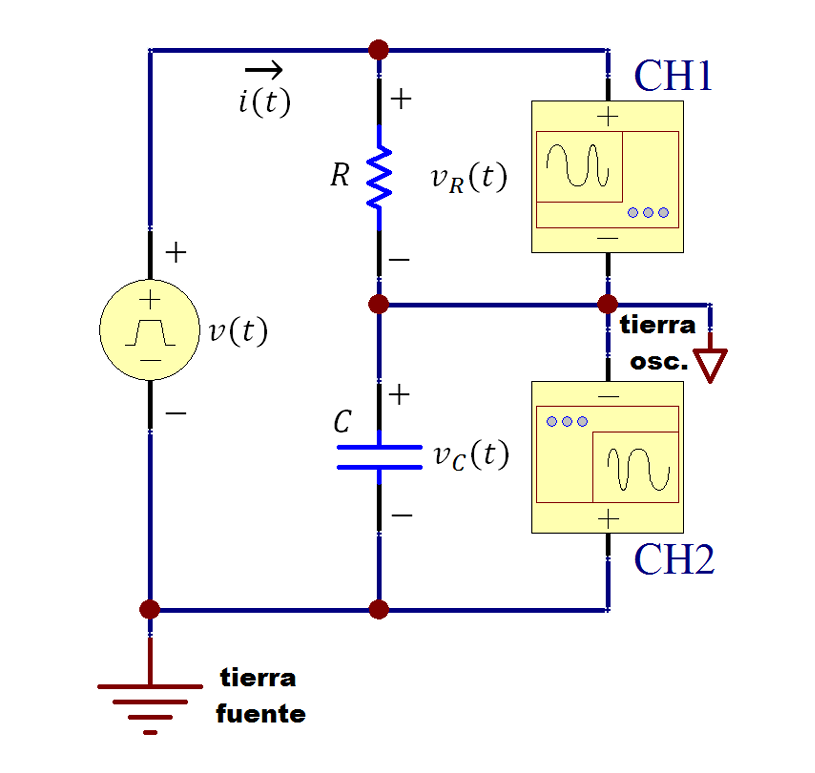
\includegraphics[width=0.48\textwidth]{circuito.png}
  \caption{Esquema del circuito RC conectado al GF y a los canales CH1 y CH2 del OSC}
  \label{fig:figura1}
  \end{figure}

%
$\pagebreak$

En el osciloscopio se ajustan las escalas y se desplazan verticalmente las funciones de tal forma que sea posible 
ver sobre el eje de tiempo los voltajes para resistencia y capacitor, luego se guardan puntos de las funciones $V_R(t)$ y $V_C(t)$, 
para carga y descarga de capacitor. Ver figura(2) para una vista general de las funciones mostradas en osciloscopio.


  %%
    \begin{figure}[ht]
    \centering
    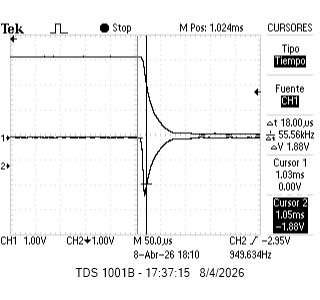
\includegraphics[width=0.48\textwidth]{vr-vc-general.jpg} %las imagenes van en pdf 
    \caption{Vista general de voltajes en funcion del tiempo para capacitor y resistencia, en este caso mientras se descarga de capacitor.}
  \label{fig:figura2}
  \end{figure}

%%
Usando los cursores del osciloscopio, se hacen varias mediciones del tiempo que tardan las funciones en variar 1/e, 
para carga será un $63\%$ del voltaje maximo ($V_{max}$) que alcanza la onda generada por GF y para descarga un $37\%$, estas serán  $\tau$ de referencia.

%A continuación se hacen los ajustes no lineales usando ecuaciones (1-4) para los puntos guardados, con tiempo como variable y $V_{max}$, $\tau$, D como parámetros, 
%siendo D el termino independiente de la función, que se agrega para mejorar el ajuste hecho con un programa de python. Ver figura(2) y figura(3).
A continuacion, para realizar los ajustes no lineales, utilizo las siguientes funciones que imitan la forma de las ecuaciones (3), (4), (5) y (6) respectivamente.
\begin{equation}V_{Cc}(x)=P_0 \left(1 - e^{-(x-x_0)/P_1}\right)+P_2\end{equation}
\begin{equation}V_{Cd}(x)=P_0 \left( e^{-(x-x_0)/P_1}\right)+P_2\end{equation}

\begin{equation}V_{Rc}(x)=P_0 \left( e^{-(x-x_0)/P_1}\right)+P_2\end{equation}
\begin{equation}V_{Rd}(x)=P_0 \left(- e^{-(x-x_0)/P_1}\right)+P_2\end{equation}
Donde $P_0$ es el voltaje maximo, $P_1$ es el tiempo caracteristico $\tau$, $P_2$ es el termino independiente que se agrega para mejorar el ajuste, 
y $x_0$ es un corrimiento en el eje de tiempo que se agrega, ya que las funciones no comienzan exactamente en $x=0s$.


%$\pagebreak$
\section{RESULTADOS}
Por medir la resistencia y capacitancia de los elementos del circuito, se aproxima un valor de tiempo característico, usando ec(7), 
$\tau_a = (0.34\pm0.01)10^{-5}s$.

Usando los $\tau$ medidos con cursores se calculan valores medios, $\overline{\tau_c}=(2.37\pm0.06)10^{-5}s$ $\overline{\tau_d}=(1.43\pm0.08)10^{-5}s$ 
para carga y descarga respectivamente.
Se realizan los ajustes no lineales para cada función (ver figuras (3) y (4)), y se rescatan los parámetros correspondientes a $\tau$ 
devueltos por el programa de ajuste, ver tabla(1).

\section{CONCLUSION}
En este trabajo se determinó el tiempo característico $\tau$ mediante tres metodos:
 el cálculo analítico ($\tau_{a}$), la medición directa con cursores ($\overline{\tau_{c}}, \overline{\tau_{d}}$) 
 y el ajuste no lineal de las curvas de voltaje.

 Al comparar los resultados de Tabla(2) se observa que los tiempos caracteristicos obtenidos por los ajustes tienen menor error relativo que 
 los calculados por los otros métodos, hallandose entre el $0.2\% $ y el $0.5\% $. Estos resultados son los más confiables del trabajo,
 ya que se ha usado una gran cantidad de puntos para el ajuste.
 Por otro lado, con los cursores se obtiene un error relativo de entre el $3\%$ y el $6\%$, debido a la gran dificultad de posicionar manualmente 
 los cursores donde correspondia, se le atribuye error humano.
   
 El valor de referencia $\tau_{a}$ calculado a partir de la resistencia y capacitancia medidas con multímetro muestra la mayor desviación respecto 
 a los valores de ajuste, que podría deberse a la inestabilidad observada en las lecturas del multímetro, el cual no mostraba un valor fijo 
 durante la medición del capacitor, afectando la precisión de $\tau_{a}$, sin mencionar que este método es el menos confiable, por basarse en mediciones que 
 tienen un error significativo, sin tener en cuenta la resistencia del cableado, que afectan el valor real de $\tau$.
 Finalmente, se concluye que el mejor método para determinar $\tau$ es el ajuste no lineal, y tomo como tiempo caracteristico final el valor medio entre estos, quedando:
 $$\tau=(1.88\pm0.01)10^{-5} s$$


%
   \begin{figure}[ht]
    \centering
    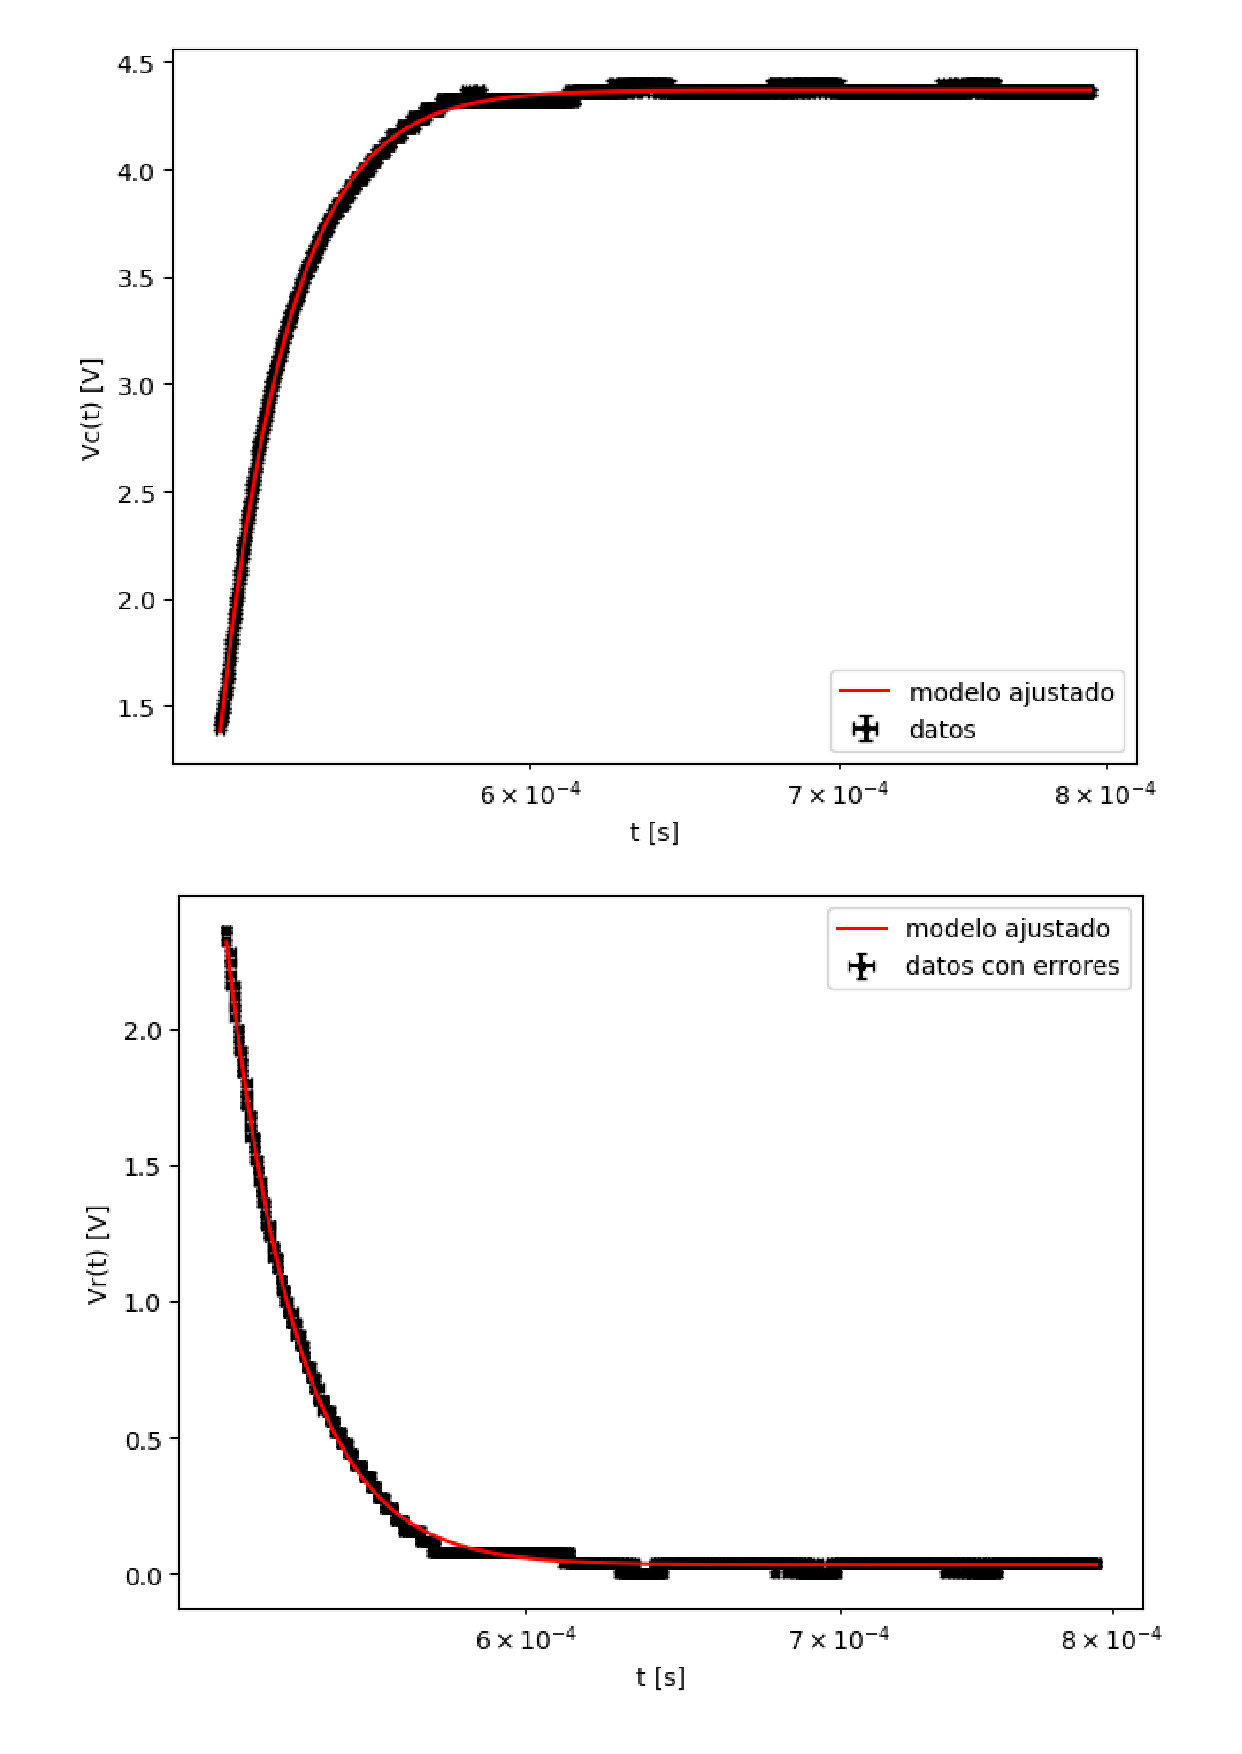
\includegraphics[width=0.48\textwidth]{carga.pdf} 
  \caption{Imagen superior: ajuste para puntos de $V_{Cc}(t)$. Imagen inferior: ajuste para puntos de $V_{Rc}(t)$. Cada punto con sus respectivas barras de error.}
  \label{fig:figura3}
  \end{figure}

  %%
    \begin{figure}[ht]
    \centering
    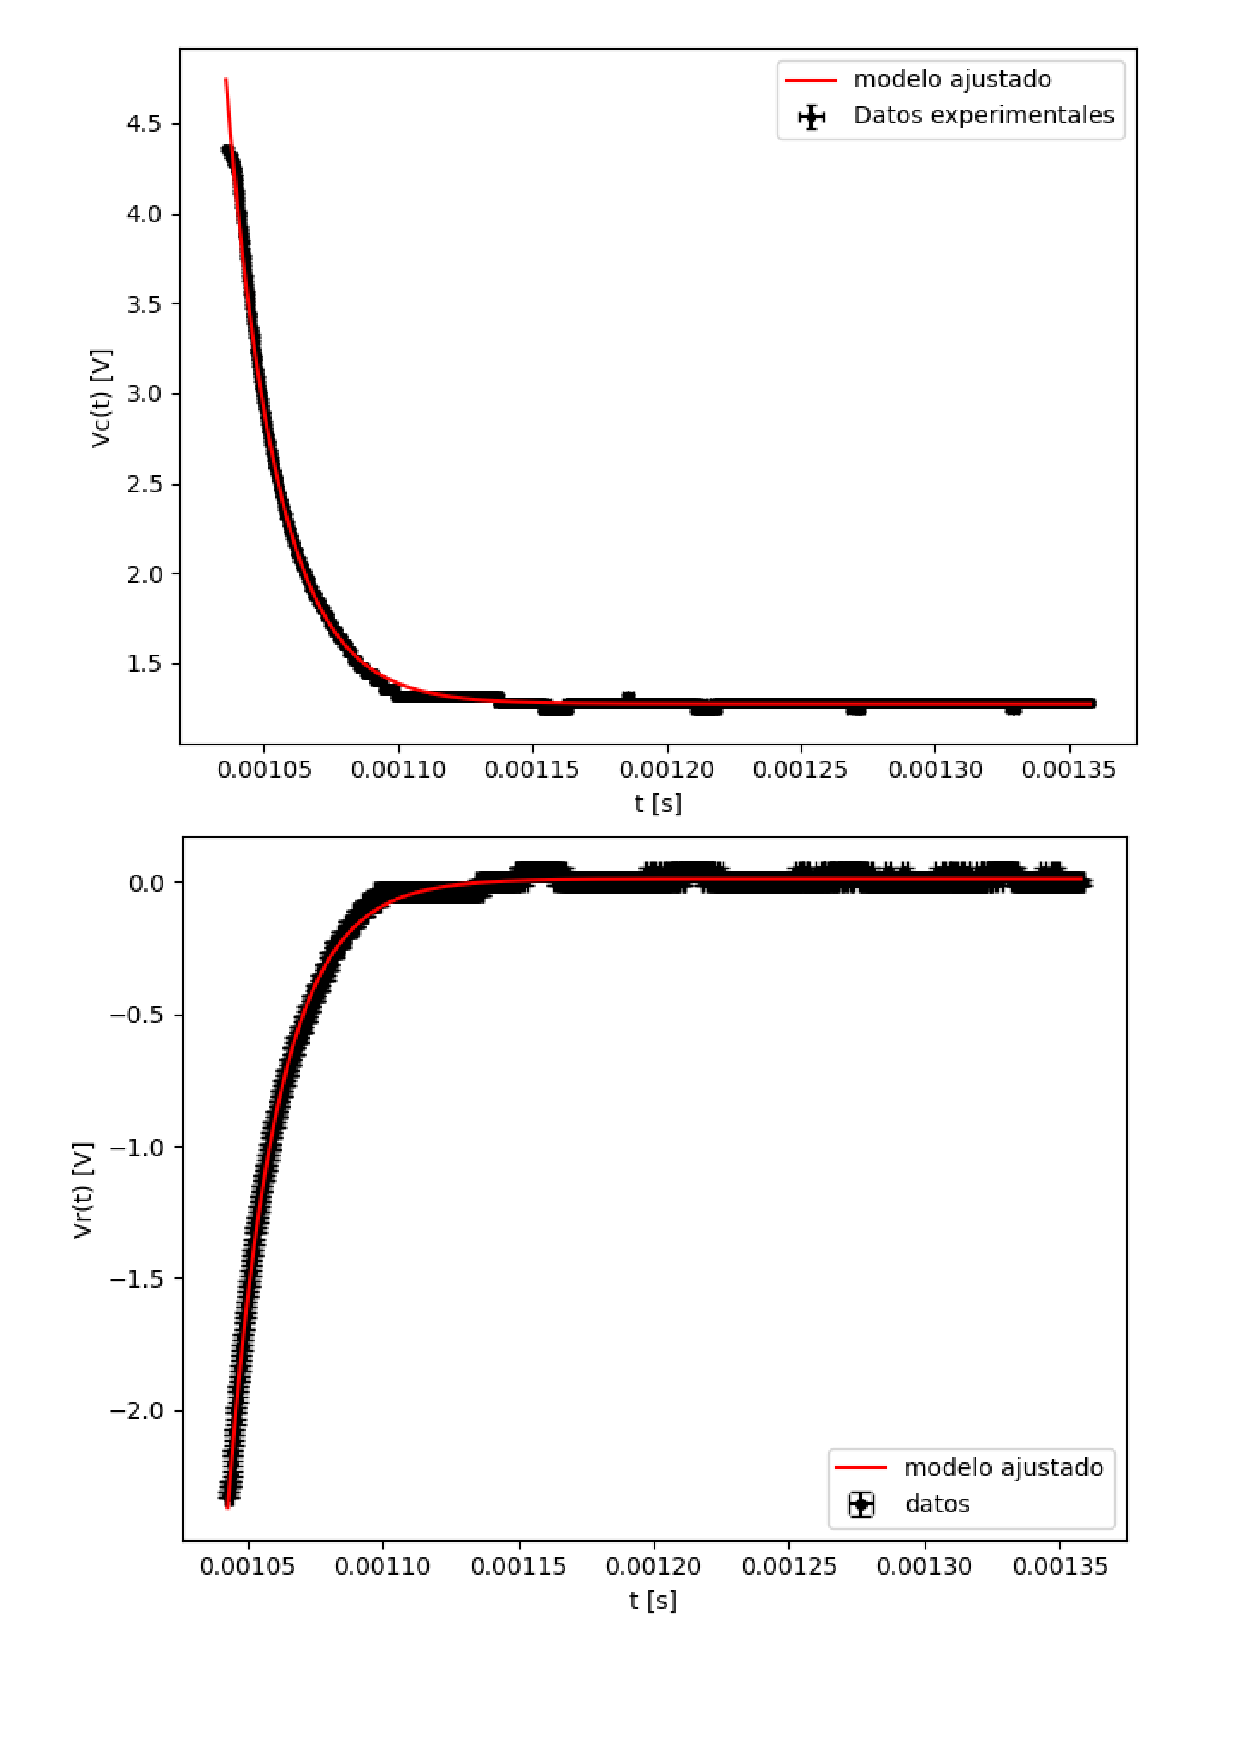
\includegraphics[width=0.48\textwidth]{descarga.pdf}
    \caption{Imagen superior: ajuste para puntos de $V_{Cd}(t)$.Imagen inferior: ajuste para puntos de $V_{Rd}(t)$. Cada punto con sus respectivas barras de error.}
  \label{fig:figura4}
  \end{figure}

%%

%tabla petit
\begin{table*}[t]  
\centering
%\caption{Estilo recomendado de tabla a doble columna}
\label{tabl:tab1}
\begin{tabular}{|c|c|c|c|c|} 
\hline
Parametros     & $V_{Cc}$ & $V_{Cd}$ & $V_{Rc}$ & $V_{Rd}$  \\ \thickhline
$P_0$ &$(2.983\pm 0.003)V$ & $(2.793\pm0.009)V$ & $(2.284\pm0.003)V$&$(-2.47\pm0.01)V$ \\ \hline
$P_1$ &$(1.778\pm0.003)10^{-5}s$ &$(1.88\pm0.01)10^{-5}s$ &$(1.814\pm0.004)10^{-5}s$ &$(2.06\pm0.01)10^{-5}s$ \\ \hline
$P_2$ &$(1.384\pm0.003)V$ &$(1.274\pm0.002)V$ &$(3.36\pm0.05)10^{-2}V$ &$(1.6\pm0.2)10^{-2}V$ \\ \hline
\end{tabular}
\caption{Parámetros obtenidos por el programa de ajuste, para cada función, de acuerdo a las ecuaciones (8-11).}
\end{table*}
%fin tabla petit
%tabla grande, ocupa el doble ancho de la página. LaTeX las ubica al principio de la hoja
\begin{table*}[t]  
\centering
%\caption{Estilo recomendado de tabla a doble columna}
\label{tabl:tab2}
\begin{tabular}{|c|c|c|}
\hline
$\tau$      & Valor hallado& $e_{relativo}(\tau)$ \\ \thickhline
$\tau_{V_Cc}$ &  $(1.778\pm0.003 )10^{-5}s$  & 0.2$\%$\\ \hline
$\tau_{V_Rc}$  &  $(1.814\pm0.004 )10^{-5}s$  & 0.2$\%$\\ \hline
$\tau_{V_Cd}$ & $(1.88\pm0.01 )10^{-5}s$ &0.5$\%$\\ \hline
$\tau_{V_Rd}$   & $(2.06\pm0.01 )10^{-5}s$ & 0.5$\%$\\ \hline
$\overline{\tau_c}$&  $(2.37\pm0.06)10^{-5}s$  & 3$\%$\\ \hline
$\overline{\tau_d}$ &  $(1.43\pm0.08)10^{-5}s$  & 6$\%$\\ \hline
$\tau_a$ &   $(0.34\pm0.01)10^{-5}s$ & 3$\%$\\ \hline
\end{tabular}
\caption{Todos $\tau$ hallados con sus errores relativos, el subinidice c o d indica que corresponde a mediciones hechas mientras se cargaba o descargaba el capacitor.}
\end{table*}




\section{REFERENCIAS}
%\vspace{-3ex}%hace
1- Guia de laboratorio:“Trabajo de 
Laboratorio Nº2: Respuesta transitoria en un circuito RC”.
Facultad de Matemática, Astronomía, 
Física y Computación 2026. Aula virtual 
Física Experimental III 2026.


2- Manual Multimetro UNI-T UT39E+


3- Manual Multimetro-LCR UNI-T UT612


4- Serway, R. A., Jewett, J. W. (2008). Física para ciencias e ingeniería (Vol. 2). Cengage Learning.

\end{document}
